\input{head-vertiefung.inc}
\usepackage{tikz-3dplot}
% Präambelbefehle für die Präsentation
\title[TET Vertiefung: Spiegelungsmethode -- Dielektrische Spiegelung]{Spiegelungsmethode -- Dielektrische Spiegelung}

\begin{document}
% 
% Frontmatter 
% 
%%%%%%%%%%%%%%%%%%%%%%%%%%%%%%%%%%%%%%%%%%%%%%%%%%%%%%%%%%%%%%%%%%%%%%%%%%%%%%%%%%%%%%%%%%%%%%%%%%%%%%%%%%%%%%%%%%%%%%%%%%%%% 

%% inserts the title page and the table of contents
\maketitle

% 
% Content 
% 
%%%%%%%%%%%%%%%%%%%%%%%%%%%%%%%%%%%%%%%%%%%%%%%%%%%%%%%%%%%%%%%%%%%%%%%%%%%%%%%%%%%%%%%%%%%%%%%%%%%%%%%%%%%%%%%%%%%%%%%%%%%%% 
\section{Spiegelung - Dielektrische Spiegelung}


\begin{frame}
  \frametitle{Problemstellung und Idee}
  \begin{itemize}[<+->]
  \item Volumen $V_2, \varepsilon_2$ eingebettet in Volumen $V_1,\varepsilon_1$
  \item Ladungen $(Q_i, \Ortsr[vs]_i)$ in $V_1$ vorgegeben.
  \item Gesucht ist die Lösung in $V_1$ \alert{und} $V_2$
  \item Lösungsidee:
    \begin{itemize}[<+->]
    \item Für die Berechnung im eingebetteten Volumen $V_1$ $\to$ Bildladungen $(Q_i^\star, \Ortsr[v]_i^\star)$ in $V_2$ als Ersatz für das eingebettete Material $\to$ $V_2$ mit $\varepsilon = \varepsilon_1$
    \item Für die Berechnung im eingebetteten Volumen $V_2$ $\to$ Bildladungen $(Q_i^{\star\star}, \Ortsr[v]_i^{\star\star})$ in $V_1$ als Ersatz für das externe Material $\to$ $V_1$ mit $\varepsilon = \varepsilon_2$
      \item Versuch: $\Ortsr[v]_i^{\star\star} = \Ortsr[vs]_i$ $\to$ Faktisch \enquote{nur} Veränderung der ursprünglichen Ladungen; keine externen Ladungen an neuen Positionen.
      \end{itemize}
    \end{itemize}
    \pause
    \begin{columns}
      \begin{column}{.3\textwidth}
      reales Problem:

      
      \begin{tikzpicture}[line width = 1.2pt, line join=round,>=stealth]
        \filldraw [color=blue!70] (2.5,2.5) circle (1pt) node[above] {$Q_i, \Ortsr[vs]_i$};
        \filldraw [color=blue!70] (2.9,2.1) circle (1pt); 
        \filldraw [color=blue!70] (2.7,1.9) circle (1pt); 
        % Ladungsdichte
        \coordinate (a) at (2.1,1.8);
        \coordinate (b) at (2,1.2);
        \coordinate (c) at (1.8,0.4);
        \coordinate (d) at (1.3,0.6);
        \coordinate (e) at (0.7,0.5);
        \coordinate (f) at (0.5,2);
        \coordinate (g) at (1.2,2.5);
        \shade[ball color=white!10!green!20,opacity=0.20] plot [smooth cycle, tension = 1] coordinates {(a) (b) (c) (d) (e) (f) (g)};
        \draw [color=darkgreen] plot [smooth cycle, tension = 1] coordinates {(a) (b) (c) (d) (e) (f) (g)} node [sloped, above] {$O(V_2)$};
        \draw(1,1.1) node {$V_2$};
        \draw(1.2,0.8) node{$\varepsilon=\varepsilon_2$};
        \draw(0,2.2) node[align=center] {$V_1$\\$\varepsilon=\varepsilon_1$}; 
      \end{tikzpicture}
        
        \end{column}
        \begin{column}{.3\textwidth}
          Berechnung in $V_1$:
      \begin{tikzpicture}[line width = 1.2pt, line join=round,>=stealth]
        \filldraw [color=blue!70] (2.5,2.5) circle (1pt) node[above] {$Q_i, \Ortsr[vs]_i$};
        \filldraw [color=blue!70] (2.9,2.1) circle (1pt); 
        \filldraw [color=blue!70] (2.7,1.9) circle (1pt); 
        \filldraw [color=red!70] (1.2,1.7) circle (1pt); 
        \filldraw [color=red!70] (1.7,1.6) circle (1pt); 
        % Ladungsdichte
        \coordinate (a) at (2.1,1.8);
        \coordinate (b) at (2,1.2);
        \coordinate (c) at (1.8,0.4);
        \coordinate (d) at (1.3,0.6);
        \coordinate (e) at (0.7,0.5);
        \coordinate (f) at (0.5,2);
        \coordinate (g) at (1.2,2.5);
        \shade[ball color=white!10!green!20,opacity=0.20] plot [smooth cycle, tension = 1] coordinates {(a) (b) (c) (d) (e) (f) (g)};
        \draw [color=darkgreen] plot [smooth cycle, tension = 1] coordinates {(a) (b) (c) (d) (e) (f) (g)} node [sloped, above] {$O(V_2)$};
        \draw(1,1.1) node {$V_2$};
        \draw(1.2,0.8) node{$\varepsilon=\varepsilon_1$};
        \draw(0,2.2) node[align=center] {$V_1$\\$\varepsilon=\varepsilon_1$}; 
        \filldraw [color=red!70] (1.3,1.9) circle (1pt) node[rectangle,fill=white,above,nearly opaque] {$-\lambda(\Ortsr[vs]_i) Q^\star_i, \Ortsr[v]^\star_i$}; 
\filldraw [color=red!70] (1.3,1.9) circle (1pt) ;
      \end{tikzpicture}
          
        \end{column}
      \begin{column}{.3\textwidth}
          Berechnung in $V_2$:
      \begin{tikzpicture}[line width = 1.2pt, line join=round,>=stealth]
        \filldraw [color=blue!70] (2.5,2.5) circle (1pt) node[above] {$Q_i, \Ortsr[vs]_i$};
        \filldraw [color=blue!70] (2.9,2.1) circle (1pt); 
        \filldraw [color=blue!70] (2.7,1.9) circle (1pt); 
        \filldraw [color=red!70] (2.5,2.5) circle (1pt);
        \filldraw [color=red!70] (2.9,2.1) circle (1pt); 
        \filldraw [color=red!70] (2.7,1.9) circle (1pt) node[below] {$Q_i^{\star\star}, \Ortsr[vs]_i$}; 

        % Ladungsdichte
        \coordinate (a) at (2.1,1.8);
        \coordinate (b) at (2,1.2);
        \coordinate (c) at (1.8,0.4);
        \coordinate (d) at (1.3,0.6);
        \coordinate (e) at (0.7,0.5);
        \coordinate (f) at (0.5,2);
        \coordinate (g) at (1.2,2.5);
        \shade[ball color=white!10!green!20,opacity=0.20] plot [smooth cycle, tension = 1] coordinates {(a) (b) (c) (d) (e) (f) (g)};
        \draw [color=darkgreen] plot [smooth cycle, tension = 1] coordinates {(a) (b) (c) (d) (e) (f) (g)} node [sloped, above] {$O(V_2)$};
        \draw(1,1.1) node {$V_2$};
        \draw(1.2,0.8) node{$\varepsilon=\varepsilon_2$};
        \draw(0,2.2) node[align=center] {$V_1$\\$\varepsilon=\varepsilon_2$}; 
      \end{tikzpicture}
        \end{column}
\end{columns}
    
\end{frame}


\begin{frame}
  \frametitle{Stetigkeitsbedingungen am Übergang}
  \begin{itemize}[<+->]
  \item \texttt{TET-Verhalten\_an\_Grenzflaechen.pdf}, \url{https://youtu.be/_SulhVuUA-Y}
  \item Normalenvektor $\vec{n}$ von Medium 1 nach Medium 2 orientiert
    \item $\vec{a} = a_n \vec{n} + a_t \frac{(\vec{n}\times \vec{a})\times\vec{n}}{\abs{\vec{n}\times \vec{a}}} = (\vec{a}\cdot\vec{n}) \vec{n} + (\vec{n}\times \vec{a})\times\vec{n}$  
  \item Induktionsgesetz $\to$ Tangentialkomponente der Elektrischen Feldstärke beim Übergang \alert{immer stetig}:
    \begin{equation*}
      \boxed{\vec{n} \times \left( \EFeld[v]_2 - \EFeld[v]_1\right) = \vec{0}} \Rightarrow \EFeld[v]_2 - \EFeld[v]_1 = (\EFeld_2\cdot\vec{n} - \EFeld_1\cdot\vec{n}) \vec{n} 
    \end{equation*}
    \item Für das Skalarpotential folgt dann mit $\EFeld[v] = -\gradient \SkalarPot$
    \begin{equation*}
      \boxed{\vec{n} \times \left( \gradient \SkalarPot_1 - \gradient \SkalarPot_2\right) = \vec{0}} \Rightarrow \gradient \SkalarPot_1 - \gradient \SkalarPot_2 = (\vec{n}\cdot\gradient \SkalarPot_1 - \vec{n}\cdot\gradient \SkalarPot_2) \vec{n}
    \end{equation*}
  \item Die Normalkomponente der Dielektrischen Verschiebung \alert{kann unstetig sein}: $\vec{n}\cdot (\DFeld[v]_2 - \DFeld[v]_1 ) = \rho_F$
  \item Hierzu muss es freie Ladungsträger geben. Für \alert{ideale Dielektrika} gilt
    \begin{equation*}
      \vec{n}\cdot (\DFeld[v]_2 - \DFeld[v]_1 ) = 0 \Rightarrow \boxed{\vec{n}\cdot (\varepsilon_2\EFeld[v]_2 - \varepsilon_1\EFeld[v]_1 ) =0 } \text{ bzw. } \boxed{\vec{n}\cdot (-\varepsilon_2\gradient\SkalarPot_2 + \varepsilon_1\gradient\SkalarPot_1 ) =0 } 
    \end{equation*}
    \item Ohne \enquote{innere Quellen} (z.B. Dipolschicht):\\ \alert{Potential zweimal stetig diff.-bar}; insbesondere $\boxed{\SkalarPot_2-\SkalarPot_1 = 0}$
    \end{itemize}
  \end{frame}


  \begin{frame}
    \frametitle{Potentiale in $V_1$ und $V_2$}
    \begin{itemize}[<+->]
    \item Greensche-Funktionen des Freiraums in $V_1$ und $V_2$:
      \begin{equation*}
        G_{\varepsilon_1}(\Ortsr[v], \Ortsr[vs]) = \frac{1}{4\pi\varepsilon_1} \frac{1}{\abs{\Ortsr[v] - \Ortsr[vs]}} \text{ bzw. }         G_{\varepsilon_2}(\Ortsr[v], \Ortsr[vs]) = \frac{1}{4\pi\varepsilon_2} \frac{1}{\abs{\Ortsr[v] - \Ortsr[vs]}} \quad G_{\varepsilon_1}= \frac{\varepsilon_2}{\varepsilon_1} G_{\varepsilon_2}  
      \end{equation*}
    \item Berechnung in $V_1$ (erstes Ersatzproblem):
      \begin{align*}
        \SkalarPot_1(\Ortsr[v]) & = Q G_{\varepsilon_1}(\Ortsr[v], \Ortsr[vs]) -  \lambda(\Ortsr[vs])Q^\star G_{\varepsilon_1}(\Ortsr[v], T(\Ortsr[vs]))\\
        & = Q G_{\varepsilon_1}(\Ortsr[v], \Ortsr[vs]) - \lambda(\Ortsr[v]) Q^\star G_{\varepsilon_1}(T(\Ortsr[v]), \Ortsr[vs])
        \end{align*}
    \item Berechnung in $V_2$ (zweites Ersatzproblem):
      \begin{align*}
        \SkalarPot_2(\Ortsr[v]) & = Q G_{\varepsilon_2}(\Ortsr[v], \Ortsr[vs]) +  Q^{\star\star} G_{\varepsilon_2}(\Ortsr[v], \Ortsr[vs])\\
                                       & = \left( Q +  Q^{\star\star}\right) G_{\varepsilon_2}(\Ortsr[v], \Ortsr[vs])
      \end{align*}
      \item Wie bei \enquote{isolierte Kugel}: Gesamtladung erhalten: $\boxed{-\lambda(\Ortsr[vs])Q^\star+Q^{\star\star}= 0}$
      \item Ziel: Bestimme $Q^\star$, $\lambda$ und $\Ortsr[v]^\star=T(\Ortsr[vs])$ so, dass die Stetigkeitsbedingungen auf $O(V_2)$ erfüllt werden. 
      \end{itemize}
    \end{frame}

    \begin{frame}
      \frametitle{Stetigkeitsbedingungen}
      \begin{itemize}[<+->]
      \item Stetigkeit des Skalarpotentials für $\Ortsr[v]\in O(V_2)$:
\begin{align*}
0 \stackrel{!}{=}  (\SkalarPot_1 - \SkalarPot_2 ) & =   Q G_{\varepsilon_1}(\Ortsr[v], \Ortsr[vs]) - \underbrace{\lambda(\Ortsr[v])}_{=1} Q^\star G_{\varepsilon_1}(\underbrace{T(\Ortsr[v])}_{=\Ortsr[v]}, \Ortsr[vs])
                                                        -\left( Q +  Q^{\star\star}\right) G_{\varepsilon_2}(\Ortsr[v], \Ortsr[vs])\\
                                                      & = \left( (Q-Q^\star) -(Q+Q^{\star\star})\frac{\varepsilon_1}{\varepsilon_2}   \right) G_{\varepsilon_1}(\Ortsr[v], \Ortsr[vs])\\
  0 &= \frac{Q-Q^\star}{\varepsilon_1} -\frac{Q+Q^{\star\star}}{\varepsilon_2} \Rightarrow \boxed{\frac{Q-Q^\star}{\varepsilon_1} = \frac{Q+Q^{\star\star}}{\varepsilon_2}}  
\end{align*}
\item Tangentialkomponente des Feldes für $\Ortsr[v]\in O(V_2)$: $\vec{n}\times (\gradient\SkalarPot_1 - \gradient\SkalarPot_2 ) =\vec{0}$
  \begin{align*}
    \vec{0} & \stackrel{!}{=} \vec{n}\times \gradient\SkalarPot_1 - \vec{n}\times \gradient\SkalarPot_2 \\
      & = \vec{n}\times \gradient \left[ Q G_{\varepsilon_1}(\Ortsr[v], \Ortsr[vs]) - \lambda(\Ortsr[v]) Q^\star G_{\varepsilon_1}(T(\Ortsr[v]), \Ortsr[vs]) \right]
        - \vec{n}\times \gradient \left[ \left( Q +  Q^{\star\star}\right) G_{\varepsilon_2}(\Ortsr[v], \Ortsr[vs]) \right]\\
      & = \vec{n}\times \gradient \left[ Q G_{\varepsilon_1}(\Ortsr[v], \Ortsr[vs]) - \lambda(\Ortsr[v]) Q^\star G_{\varepsilon_1}(T(\Ortsr[v]), \Ortsr[vs]) \right]
        - \vec{n}\times \gradient \left[ \left( Q +  Q^{\star\star}\right) \frac{\varepsilon_1}{\varepsilon_2} G_{\varepsilon_1}(\Ortsr[v], \Ortsr[vs]) \right]
    \end{align*}
  \end{itemize}
      \end{frame}

   \begin{frame}
     \frametitle{Stetigkeitsbedingungen (fortgeführt)}
     \begin{equation*}
       \vec{0}= \vec{n}\times \gradient \left[ Q G_{\varepsilon_1}(\Ortsr[v], \Ortsr[vs]) - \lambda(\Ortsr[v]) Q^\star G_{\varepsilon_1}(T(\Ortsr[v]), \Ortsr[vs]) \right]
        - \vec{n}\times \gradient \left[ \left( Q +  Q^{\star\star}\right) \frac{\varepsilon_1}{\varepsilon_2} G_{\varepsilon_1}(\Ortsr[v], \Ortsr[vs]) \right]
       \end{equation*}
      \begin{itemize}[<+->]
      \item Auf $\lambda$ und $T$ wird der Gradient angewendet. Es kann nicht einfach $\lambda(\Ortsr[v])=1$ und $T(\Ortsr[v])=\Ortsr[v]$ für $\Ortsr[v]\in O(V_2)$ verwendet werden.
      \item Weiterrechnen:
        \begin{align*}
          \vec{0} &= Q \; \vec{n}\times \gradient G_{\varepsilon_1}(\Ortsr[v], \Ortsr[vs]) - Q^\star\; \vec{n}\times\gradient\left( \lambda(\Ortsr[v]) G_{\varepsilon_1}(T(\Ortsr[v]), \Ortsr[vs]) \right)\\
            &\quad - \left( Q +  Q^{\star\star}\right) \frac{\varepsilon_1}{\varepsilon_2}\; \vec{n}\times \gradient  G_{\varepsilon_1}(\Ortsr[v], \Ortsr[vs]) \\
            &= \left( Q  - \left( Q +  Q^{\star\star}\right) \frac{\varepsilon_1}{\varepsilon_2} \right)\; \vec{n}\times \gradient G_{\varepsilon_1}(\Ortsr[v], \Ortsr[vs]) - Q^\star\; \vec{n}\times\gradient\left( \lambda(\Ortsr[v]) G_{\varepsilon_1}(T(\Ortsr[v]), \Ortsr[vs]) \right)\\
            &= \left( Q  - \left( Q +  Q^{\star\star}\right) \frac{\varepsilon_1}{\varepsilon_2} \right)\; \vec{n}\times \gradient G_{\varepsilon_1}(\Ortsr[v], \Ortsr[vs])  \\
            &\quad - Q^\star G_{\varepsilon_1}(T(\Ortsr[v]), \Ortsr[vs])\; \vec{n}\times\gradient \lambda(\Ortsr[v]) - Q^\star\lambda(\Ortsr[v]) \; \vec{n}\times\gradient G_{\varepsilon_1}(T(\Ortsr[v]), \Ortsr[vs]) \\
          &= \left( Q  - \left( Q +  Q^{\star\star}\right) \frac{\varepsilon_1}{\varepsilon_2} \right)\; \vec{n}\times \gradient G_{\varepsilon_1}(\Ortsr[v], \Ortsr[vs])  \\
          &\quad - Q^\star G_{\varepsilon_1}(\Ortsr[v], \Ortsr[vs])\; \vec{n}\times\gradient \lambda(\Ortsr[v]) - Q^\star \; \vec{n}\times\gradient G_{\varepsilon_1}(T(\Ortsr[v]), \Ortsr[vs])
        \end{align*}
 \end{itemize}
      \end{frame}


      \begin{frame}
     \frametitle{Stetigkeitsbedingungen (fortgeführt)}
        \begin{equation*}
          {\scriptstyle \vec{0} = \left( Q  - \left( Q +  Q^{\star\star}\right) \frac{\varepsilon_1}{\varepsilon_2} \right)\; \vec{n}\times \gradient G_{\varepsilon_1}(\Ortsr[v], \Ortsr[vs])  
          - Q^\star G_{\varepsilon_1}(\Ortsr[v], \Ortsr[vs])\; \vec{n}\times\gradient \lambda(\Ortsr[v]) - Q^\star \; \vec{n}\times\gradient G_{\varepsilon_1}(T(\Ortsr[v]), \Ortsr[vs])}
        \end{equation*}
      \begin{itemize}[<+->]
      \item $T$ stetig diff.-bar und $T(T(\Ortsr[v]))=\Ortsr[v]$ : $\gradient_{\Ortsr[v]} G_{\varepsilon_1}(T(\Ortsr[v]), \Ortsr[vs])  = \gradient_{T(\Ortsr[v])} G_{\varepsilon_1}(T(\Ortsr[v]), \Ortsr[vs])$
        \item Damit lässt sich der Ausdruck weiter zusammenfassen:
        \begin{align*}
          \vec{0} &= \underbrace{\left( \left(Q - Q^\star\right) - \left( Q +  Q^{\star\star}\right) \frac{\varepsilon_1}{\varepsilon_2} \right)}_{=0}\; \vec{n}\times \gradient G_{\varepsilon_1}(\Ortsr[v], \Ortsr[vs])   - Q^\star G_{\varepsilon_1}(\Ortsr[v], \Ortsr[vs])\; \vec{n}\times\gradient \lambda(\Ortsr[v]) 
        \end{align*}
      \item Somit gilt für $\Ortsr[v]\in O(V_2)$:
        \begin{equation*}
          \boxed{\vec{n}\times\gradient \lambda(\Ortsr[v]) = \vec{0}}
          \end{equation*}

     \item Führt man gleichen Operationen mit der Stetigkeitsbedingung für die Normalkomponente durch, so gilt für $\Ortsr[v]\in O(V_2)$ auch:
        \begin{equation*}
          \boxed{\vec{n}\cdot\gradient \lambda(\Ortsr[v]) = 0}
          \end{equation*}
 \item Insgesamt gilt also für $\Ortsr[v]\in O(V_2)$:
        \begin{equation*}
          \boxed{\gradient \lambda(\Ortsr[v]) = \vec{0}}
          \end{equation*}
        \end{itemize}
      \end{frame}

 \begin{frame}
     \frametitle{Zusammenfassung}
     \begin{itemize}[<+->]
     \item Aus der Konstanz der Gesamtladung:
       \begin{equation*}
          \boxed{-\lambda(\Ortsr[vs])Q^\star+Q^{\star\star}= 0}
       \end{equation*}
      \item Aus der Stetigkeit des Potentials für $\Ortsr[v]\in O(V_2)$:
        \begin{equation*}
          \boxed{\frac{Q-Q^\star}{\varepsilon_1} = \frac{Q+Q^{\star\star}}{\varepsilon_2}}
       \end{equation*}
     \item Aus Normal- und Tangentialkomponente des Feldes für $\Ortsr[v]\in O(V_2)$:
       \begin{equation*}
         \boxed{\gradient \lambda(\Ortsr[v]) = \vec{0}}
       \end{equation*}
     \item Keine allgemeine Lösung. Aber $\lambda (\Ortsr[v]) = 1$ (Ebene, Zylinder) erfüllt die letzte Beziehung.
     \item Mit $\lambda (\Ortsr[v]) = 1$:
       \begin{equation*}
         Q^\star = Q^{\star\star} \text{ und } \frac{Q-Q^\star}{\varepsilon_1} = \frac{Q+Q^{\star}}{\varepsilon_2} \Rightarrow \boxed{Q^\star = \frac{\varepsilon_2-\varepsilon_1}{\varepsilon_2+\varepsilon_1} Q}
         \end{equation*}
         
       \end{itemize}
 \end{frame}

 \begin{frame}
   \frametitle{Dielektrische Spiegelung an der Ebene}
   \begin{columns}
     \begin{column}{.35\textwidth}
     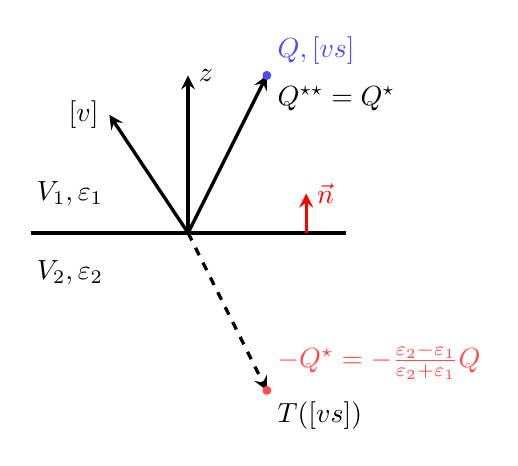
\begin{tikzpicture}[line width = 1.2pt, line join=round,>=stealth]
       \coordinate (O) at (0,0);
       \coordinate (a) at (-2,0);
       \coordinate (b) at (2,0);
       \draw (a) -- (b);
       \draw[color=red, -stealth] (1.5,0) -- (1.5,.5) node[right] {$\vec{n}$}; 
       \draw[ -stealth] (O) -- (0,2) node[right] {$z$}; 
       \draw[ -stealth] (O) -- (-1,1.5) node[left] {$\Ortsr[v]$}; 
       \draw[ -stealth] (O) -- (1,2) node[below right] {$Q^{\star\star}=Q^\star$};
       \filldraw [color=blue!70] (1,2) circle (1pt) node[above right] {$Q, \Ortsr[vs]$}; 
       \draw[ dashed, -stealth] (O) -- (1,-2) node[below right] {$T(\Ortsr[vs])$};
       \filldraw [color=red!70] (1,-2) circle (1pt) node[above right] {$-Q^\star=-\frac{\varepsilon_2-\varepsilon_1}{\varepsilon_2+\varepsilon_1} Q$}; 
\draw(-1.5,0.5) node {$V_1,\varepsilon_1$}; 
\draw(-1.5,-0.5) node {$V_2,\varepsilon_2$}; 

\end{tikzpicture}
       \end{column}
       \begin{column}{.65\textwidth}
         \begin{itemize}[<+->]
           \item In $V_1$:
      \begin{align*}
        \SkalarPot_1(\Ortsr[v]) & = Q G_{\varepsilon_1}(\Ortsr[v], \Ortsr[vs]) -  Q^\star G_{\varepsilon_1}(\Ortsr[v], T(\Ortsr[vs]))\\
        & = Q\left( G_{\varepsilon_1}(\Ortsr[v], \Ortsr[vs]) -  \frac{\varepsilon_2-\varepsilon_1}{\varepsilon_2+\varepsilon_1} G_{\varepsilon_1}(\Ortsr[v], T(\Ortsr[vs]))\right)\\
        & = Q\frac{\varepsilon_0}{\varepsilon_1}\left( G(\Ortsr[v], \Ortsr[vs]) -  \frac{\varepsilon_2-\varepsilon_1}{\varepsilon_2+\varepsilon_1} G(\Ortsr[v], T(\Ortsr[vs]))\right)
        \end{align*}
    \item In $V_2$:
      \begin{align*}
        \SkalarPot_2(\Ortsr[v]) & = Q G_{\varepsilon_2}(\Ortsr[v], \Ortsr[vs]) +  Q^{\star\star} G_{\varepsilon_2}(\Ortsr[v], \Ortsr[vs])\\
                                       & = Q \left( 1 +  \frac{\varepsilon_2-\varepsilon_1}{\varepsilon_2+\varepsilon_1}\right) G_{\varepsilon_2}(\Ortsr[v], \Ortsr[vs]) \\
                                       & = Q\frac{\varepsilon_0}{\varepsilon_2} \left( 1 +  \frac{\varepsilon_2-\varepsilon_1}{\varepsilon_2+\varepsilon_1}\right) G(\Ortsr[v], \Ortsr[vs]) \\
                                       & = Q\frac{\varepsilon_0}{\varepsilon_1} \left( 1 -  \frac{\varepsilon_2-\varepsilon_1}{\varepsilon_2+\varepsilon_1}\right) G(\Ortsr[v], \Ortsr[vs]) 
      \end{align*}
          \end{itemize}
       \end{column}
     \end{columns}
\end{frame}      
\input{finalframe.inc}
\end{document}